\immediate\write18{makeindex -s nomencl.ist -o rapport.nls rapport.nlo}

\documentclass[11pt]{article}

%Langue et encodage :
 \usepackage[T1]{fontenc}
 \usepackage[utf8]{inputenc}
 \usepackage{lmodern}
 \usepackage[french]{babel} \usepackage{lmodern}


%Mise en page
\usepackage[a4paper, margin=2.5cm]{geometry}	%Papier
\usepackage{arev}									%Police
\renewcommand{\baselinestretch}{1.15} 				%Interligne
\setlength\parindent{4pt}							%Alineas
\usepackage[skip=5pt,font=footnotesize]{caption}
\usepackage{float}
\usepackage{xcolor}									%Couleurs perso
\definecolor{grisPerso}{rgb}{0.9,0.9,0.9}
\usepackage{tabu}

%Contenu :
\usepackage{hyperref}								%Liens
\usepackage{amsmath}								%Math
\usepackage{listings}								%Code source
\lstset{
language=bash,
backgroundcolor=\color{grisPerso},
basicstyle=\footnotesize,
frame=single}
\usepackage[refpage]{nomencl}						%Nomenclature
\usepackage{xpatch}
\makenomenclature

%Dessins et schémas
\usepackage{graphicx}
\usepackage{epstopdf}
\epstopdfsetup{outdir=./}
\usepackage{tikz}
\usepackage{includes/tikz-uml}
\usetikzlibrary{positioning,chains,fit,shapes,calc}
\newcommand{\illu}[3]{%
	\begin{figure}[ht!]
			  \centering
			  \includegraphics[scale=#3]{Graphics/#1}
			  \caption{#2}
			  \smallskip
	\end{figure}}

\newcommand*\emptyPage{\newpage\null\thispagestyle{empty}\newpage}

\begin{document}

\begin{titlepage}
\newgeometry{top=2cm,bottom=2cm}

\newcommand{\HRule}{\rule{\linewidth}{0.5mm}} % Defines a new command for the horizontal lines, change thickness here

\center % Center everything on the page
 
%----------------------------------------------------------------------------------------
%   HEADING SECTIONS
%----------------------------------------------------------------------------------------


\includegraphics[scale=0.6]{Graphics/logo.png}\\[1.5cm]

\textsc{\Large Projet Electif (technique)}\\[0.5cm] % Major heading such as course name
\textsc{\large Projet technique}\\[0.5cm] % Minor heading such as course title

{\normalsize \today}\\[1.5cm]

%----------------------------------------------------------------------------------------
%   TITLE SECTION
%----------------------------------------------------------------------------------------

\HRule \\[0.4cm]
{ \Large \bfseries Evolution de véhicules autonomes dans un environnement urbain intelligent}\\[0.4cm] % Title of your document
\HRule \\[2.5cm]


%----------------------------------------------------------------------------------------
%   LOGO SECTION
%----------------------------------------------------------------------------------------

 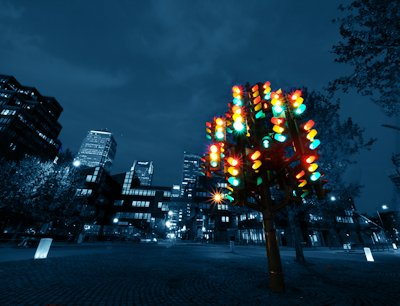
\includegraphics[scale=0.45]{Graphics/illustration.jpg}\\[2.5cm]

%----------------------------------------------------------------------------------------
%   AUTHOR SECTION
%----------------------------------------------------------------------------------------
{\normalsize Auteurs:}\\
\small
\textsc{Biton} Guillaume (guillaume.biton@ipsa.fr)\\
\textsc{Guichard} Marc-Antoine \small(marc-antoine.guichard@ipsa.fr)\\
\textsc{Lhermite} Camille \small(camille.lhermite@ipsa.fr)\\
\textsc{Monnot} Maxime \small(marc-antoine.guichard@ipsa.fr)\\[1cm]

 
%----------------------------------------------------------------------------------------

\vfill % Fill the rest of the page with whitespace

\restoregeometry

\end{titlepage}

\newpage
\tableofcontents
\newpage
\pagenumbering{arabic}

\section{Introduction}

	La voiture autonome, loin du concept de science-fiction qu'elle pouvait représenter il y a quelques années est en train de devenir une réalité.\\

Si cette ambition put être à une certaine époque motivée par le simple attrait de la prouesse technique, nous percevons aujourd'hui tous les bénéfices que l'on pourrait en tirer.
En effet, les avancées scientifiques et techniques nous permettent désormais de prétendre à concevoir une voiture qui soit non seulement autonome, mais surtout intelligente. Il est aujourd'hui tout à fait réaliste de penser que dans les quelques années à venir les voitures sauront adopter un comportement bien plus intelligent que celui de leurs conducteurs actuels, et ce au profit de la sécurité, de l' efficience énergétique mais également de l'encombrement des axes routiers.\\

A terme, nous pouvons facilement imaginer que les différents véhicules auront la possibilité de communiquer entre eux afin de prévenir les véhicules environnants de leurs intentions, mais cela ne les dispensera pas de devoir être capables d'évaluer leur environnement afin d'y détecter les éléments "indépendants" (piétons, obstacles...). \\

Comme toute révolution technologique, la voiture intelligente devra faire face au caractère progressif de son adoption: toutes les voitures sur les routes ne deviendront pas autonomes du jour au lendemain. Ces véhicules devront donc également être capables d'évoluer au milieu d'une circulation telle que nous la connaissons, où chaque acteur adopte un comportement presque parfaitement aléatoire, et ne signale pas toujours ces intentions.\\

Si les voitures deviennent intelligentes, c'est également le cas, depuis quelques années déjà, de la signalisation. Ainsi, de plus en plus de feux adaptent leur comportement au trafic, ce qui s'inscrit également dans une démarche d'optimisation de la circulation. Il est très réaliste d'espérer que cette technologie déjà existante se fera omniprésente dans les années qui viennent, d'où notre volonté d'inclure cet élément d’environnement à notre projet.\\

Le but de ce projet est donc d'étudier notre capacité à faire cohabiter intelligence artificielle et environnement "réel" et indépendant avec des moyens techniques et financiers extrêmement restreints, mais également et surtout de fournir une plateforme d'expérimentation aux étudiants de l'IPSA (et d'ailleurs ?) afin de faciliter l'apprentissage des sciences de la mécatronique et de l’intelligence artificielle tout en ancrant ce savoir dans une réalité pratique et stimulante.

\newpage
\section{Définition du besoin}

	Une définition pertinente du besoin est une condition absolument nécessaire pour la bonne réalisation de tout projet. Nous nous emploierons donc à définir aussi précisément et pertinemment que possible le besoin motivant ce projet, et à régulièrement revenir sur ce dernier afin de prendre en compte d'éventuelles évolutions et à prévenir toute dérive du projet.

\subsection{Besoin}
Le besoin à l'origine de ce projet fut exprimé par mesdames A. Belbachir et S. Benabid en tant qu'enseignants chercheurs au laboratoire Mécatronique, Signal et Systèmes à l'IPSA. Leur souhait était de bénéficier d'une plateforme articulée autour de robots autonomes évoluant dans une simulation d’environnement urbain, capables de détecter des feux de signalisation "intelligents" et d'adapter leur comportement en conséquence. Cette plateforme pourrait servir de support de TP\nomenclature{TP}{Travaux Pratiques} dans l'ensemble des matières enseignées par le département, mais également servir de "vitrine" voir même de plateforme de recherche.\\

Les principales fonctionnalités évoquées étant :
\begin{itemize}
	\item \textbf{La reconnaissance d'image} pour la détection des feux de signalisation.
	\item \textbf{La présence de feux bicolores commandés par FPGA\nomenclature{FPGA}{PGA (Field-Programmable Gate Array, ou Réseau de Portes Programmables : un type très répandu de circuit logiques programmables.}.} Ces feux seraient "intelligents" dans le sens où il s'adapteraient à la circulation. La présence de capteurs de présence est donc induite.
\end{itemize}

\subsection{Précision du besoin}

Ayant suivi nombre de matières enseignées par le département et participé à de nombreuses séances de travaux pratiques, nous bénéficions d'une image relativement claire des implications de ce projet ainsi que des contraintes relevant pour la plupart du simple bon sens.
Dans un soucis de clarté et d'application de "bonnes pratiques" nous prîmes cependant soin de valider l'ensemble de ces éléments au cours de réunions avec nos "clients" du laboratoire.\\

Ainsi, nous ajoutâmes les points suivants à la liste des exigences :
\begin{itemize}
	\item "Côté circuit" :
	\begin{itemize}
		\item \textbf{Le circuit devra bénéficier d'un encombrement raisonnable}.
		\item \textbf{Les feux de circulation devront pouvoir être commandés via une carte FPGA}.
	\end{itemize}
	\item "Côté robots" :
	\begin{itemize}
		\item \textbf{Les robots devront pouvoir être utilisés en classe sans que les préoccupations matérielles ne soient accaparantes}.
		\item \textbf{Les robots devront pouvoir être programmés en utilisant les langages enseignés à l'IPSA} à savoir C et C++ et ses variantes (Arduino...), Python, voir même Matlab...
		\item \textbf{Les robots devront bénéficier de possibilités d'application flexibles :} les enseignements étant ciblés, il est important que les utilisateurs des robots puissent se concentrer sur un aspect de leur utilisation sans avoir à se soucier des autres. De même, les robots devront embarquer suffisamment de capteurs ou tout du moins de capacité d'extensions pour que cela ne soit pas un facteur limitant lors de l'élaboration de sujets de TP.
		\item \textbf{Les robots devront ne pas pouvoir représenter un danger pour ses utilisateurs}.
	\end{itemize}
\end{itemize}
	
	\nomenclature{SCL}{Serial Clock}

	\illu{Schematic.png}{Basic input/output schematic}{0.45}

\newpage
\section{Ebauche de solution}

	Nous pouvons d'ores et déjà ébaucher les diagrammes des cas d'utilisation de haut niveau suivants :

\subsection{Pour le robot :}

	\begin{tikzpicture} 
		\begin{umlsystem}[x=10, fill=blue!10]{Robot} 
		\umlusecase[fill=white]{Charger un programme} 
		\umlusecase[y=-2,fill=white]{Evoluer en autonomie} 
		\umlusecase[y=-4,fill=white]{Changer la batterie} 
		\end{umlsystem} 
		 
		\umlactor{Développeur}  
		\umlactor[y=-3]{Utilisateur} 
		   
		\umlinherit{Développeur}{Utilisateur} 
		\umlassoc{Développeur}{usecase-1} 
		\umlassoc{Utilisateur}{usecase-2} 
		\umlassoc{Utilisateur}{usecase-3}	 
	\end{tikzpicture} 

	\textbf{Reprogrammation :}
	\begin{itemize}
		\item \textbf{Précondition :} Nous disposons d'un programme fonctionnel.
		\item \textbf{Déclencheur :} Un développeur souhaite implémenter un programme.
		\item \textbf{Scenario :}
		\begin{enumerate}
			\item On connecte le robot à une source de tension.
			\item On établit une liaison entre le robot et un ordinateur.
			\item Le développeur lance le téléversement du programme.
			\item Le robot acquitte.
			\item On ferme la connexion.
		\end{enumerate}
	\end{itemize}

	\textbf{Evolution en autonomie:}
	\begin{itemize}
		\item \textbf{Précondition :} Le robot a été programmé et dispose d'une batterie chargée.
		\item \textbf{Déclencheur :} Un membre du laboratoire souhaite observer le comportement du robot.
		\item \textbf{Scenario :}
		\begin{enumerate}
			\item On met le robot sous tension.
			\item On place le robot sur une ligne blanche du circuit.
			\item On appuie sur le bouton de démarrage de séquence
			\item Le robot déclenche les programmes en mémoire.
		\end{enumerate}
	\end{itemize}

	\textbf{Changement de batterie:}
	\begin{itemize}
		\item \textbf{Déclencheur :} On souhaite changer la batterie du robot
		\item \textbf{Scenario :}
		\begin{enumerate}
			\item On met le robot hors tension.
			\item On accède à la batterie en place le cas échéant, et on la retire.
			\item On met en place la nouvelle batterie
			\item On remet en place les éléments éventuellement retirés pour accéder à la batterie.
		\end{enumerate}
	\end{itemize}


	Le mode d'utilisation primaire est bien évidemment celui de l'évolution en autonomie. Le robot étant destiné à servir de plateforme de recherche, et devant donc être entièrement reprogrammable, il est délicat de décrire ce mode d'utilisation qui dépendra intégralement du programme chargé par l'utilisateur.\\

	Nous nous appliquerons cependant à décrire le mode d'utilisation correspondant à l'application la plus basique du robot, mais également au programme livré avec ce dernier.
\subsection{Pour le circuit :}

	\begin{tikzpicture} 
		\setcounter{tikzumlUseCaseNum}{0}
		\begin{umlsystem}[x=10, fill=blue!10]{Circuit} 
		\umlusecase[fill=white]{Charger un programme} 
		\umlusecase[y=-2,fill=white]{Evoluer en autonomie}  
		\end{umlsystem} 
		 
		\umlactor[y=0.5]{Développeur}  
		\umlactor[y=-2.5]{Utilisateur} 
		   
		\umlinherit{Développeur}{Utilisateur} 
		\umlassoc{Développeur}{usecase-1} 
		\umlassoc{Utilisateur}{usecase-2}  
	\end{tikzpicture}


\newpage
\section{Subdivision du problème}

	\subsection{Suivi de trajectoire}

Dans un soucis d’offrir une capacité de suivi de trajectoire simple et robuste, il a été décidé d’intégrer au robot une capacité de suivi de ligne blanche. Il s’agit de l’une des méthodes les plus répandues, relativement simple à implémenter et économe aussi bien en composants qu’en puissance de calcul nécessaire.\\

L’idée est d’offrir une basse fiable et simple pour que le suivi de trajectoire ne soit pas une source de préoccupation, ou d’erreur pour un chercheur qui s’intéresserait à d’autres problématiques. Cela n’exclut cependant pas qu’un chercheur désireux d’explorer d’autres possibilités de suivi de trajectoire (via la caméra, un dispositif de triangulation ou autre) de désactiver ce module et d’exploiter une autre solution.\\

Le principe de suivi de ligne est relativement simple : on place sur l’axe du robot, quelques millimètres au-dessus du sol, un capteur appelé « réflecteur optique ». Ce capteur émet une onde lumineuse (souvent infrarouge) et une cellule mesure l’intensité reçue sur la longueur d’onde émise. Une forte intensité reçue indiquera la présence d’une surface réfléchissante, tandis qu’une faible intensité indiquera la présence d’une surface absorbante. Il est ainsi aisé de différencier un fond sombre (la « route ») d’une ligne blanche.\\

Une loi linéaire lie la tension lue en sortie de capteur à l'intensité reçue.\\
Une simple lecture de cette tension permet, après comparaison avec des valeurs "seuil" définies expérimentalement, de savoir si le capteur se trouve au dessus d'une ligne blanche ou non.\\

\begin{figure}[ht!]
	\centering
	\begin{minipage}{0.48\textwidth}
		\centering
		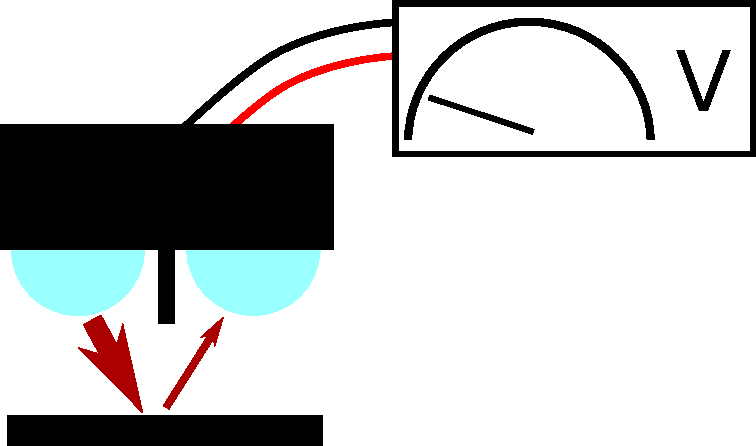
\includegraphics[scale=0.45]{Graphics/capteurOptiqueFondNoir.pdf}
		\caption{Capteur au dessus d'un support sombre}
	\end{minipage}\hfill
	\begin{minipage}{0.48\textwidth}
		\centering
		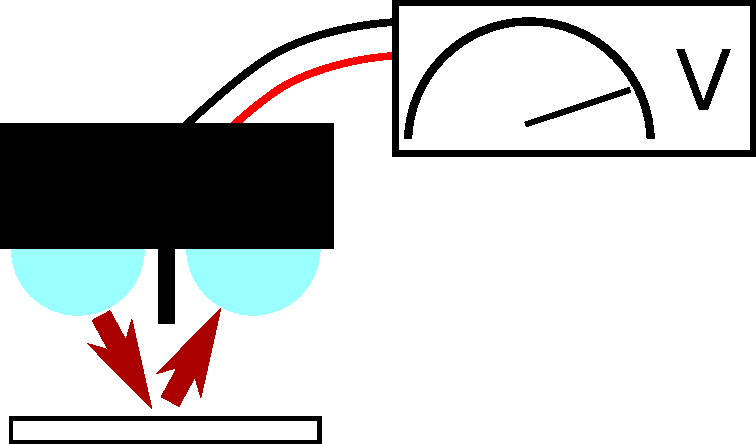
\includegraphics[scale=0.45]{Graphics/capteurOptiqueFondBlanc.pdf}
		\caption{Capteur au dessus d'un support clair}
	\end{minipage}
\end{figure}

La question qui se pose est celle du nombre de capteurs, et de leur disposition.\\

Il est tout à fait possible de n'utiliser qu'un capteur : chaque fois qu'il quite la ligne blanche, on entammera un virage à droite (puis à gauche si on ne retrouve pas la ligne blanche dans les quelques millisecondes suivantes) jusqu'à retrouver la ligne. Il est évident que cette méthode ne permettra pas une très grande fluidité de déplacement pour notre robot.\\

L'utilisation de deux capteurs permet une meilleure fluidité. On placera cette fois un capteur de chaque côté de la ligne.

\newpage
\section{Retour à une vue d'ensemble}

	\input{chapitres/4_vueEnsemble}

\newpage
\section{Estimation du coût}

	\input{chapitres/5_estimationCout}

\newpage
\section{Conclusion}
	
	\input{chapitres/6_conclusion}

\setcounter{secnumdepth}{0}
\renewcommand{\thesubsection}{\Alph{subsection}}

\newpage
\sectionWoNum{Annexes}

	\subsection{Annexe 1}

\setcounter{secnumdepth}{0}
\newpage
\section{Références}

	\subsection{Nomenclature}
		\printnomenclature

	\newpage
	\subsection{Bibliographie}
		\begingroup
		\renewcommand{\section}[2]{}%
		\bibliography{bibliography}{}
		\bibliographystyle{plain}
		\endgroup

	\newpage
	\subsection{Table des illustrations}
		\begingroup
		\renewcommand{\section}[2]{}%
		\listoffigures
		\endgroup

\newpage
\section{Résumé}
\end{document}